%Sustitucion de IEEEeqnarray
\graphicspath{ {img/BD/} }
\chapter[Background Detection of Primary User Activity in Opportunistic Spectrum Access][Background Detection of Primary User Activity in OSA]{Background Detection of Primary User Activity in Opportunistic Spectrum Access}\label{BD_chap}
\section{Introduction}\label{BD_sec_intro}
\subsection{Motivation}
One of the main problems of opportunistic spectrum access, OSA, is that current radio frequency front-ends cannot perform sensing and transmission in the same channels at the same time. In consequence, in OSA protocols, spectrum sensing and SU data transmission are performed in two separated phases. The scanning phase allows the SUs to find spectrum holes to transmit in.
However, during the transmission phase, a channel occupied by an SU can be eventually used by a PU transmission (transmission overlap) causing a potentially harmful interference to the PU receiver.
To solve this problem, the SU is only allowed to transmit during a limited amount of time after which it leaves the channel or performs a new sensing procedure (periodic sensing).

OSA with periodic sensing (\cite{ref:TransSignalProc}, \cite{ref:JSAC2007}, \cite{ref:TransWire2008}, \cite{ref:TransWire2009}, \cite{ref:TransWireOct2008}, \cite{ref:TransWire2012}) consists of a sensing period followed by a transmission period. These two separated periods are sometimes referred to as the medium access control (MAC) frame. In general, a longer sensing duration improves the sensing quality, but the higher sensing overhead in the MAC frame reduces SU throughput. The duration of the transmission period has also influence on the SU throughput and the probability of collision with PU transmissions. The throughput-collision tradeoff is present in \cite{ref:TransSignalProc} and \cite{ref:JSAC2007}, where joint designs of the sensing and access strategy are proposed. For a fixed frame duration, \cite{ref:TransWire2008} optimizes the sensing time to improve the SU throughput under detection quality constraints. In contrast, \cite{ref:TransWire2009} considers a fixed sensing time and optimizes the transmission duration subject to an interference power constraint. Both sensing and transmission times were jointly optimized in \cite{ref:TransWireOct2008} and \cite{ref:TransWire2012}. One of the main contributions of the latter is to consider the impact of imperfect sensing on the throughput of secondary users as well.

The OSA model of these works constitute the base upon which we develop our proposal. We assume a system in which the sensing period is long enough to find, with a sufficiently high reliability, an available channel to transmit in. According to a given PU activity model, the length of the SU transmission period is set to the value that maximizes the SU throughput under the desired collision probability constraint. This is a worst case PU QoS criteria used in multiple previous works (\cite{ref:JSAC2007}, \cite{ref:TransWire2012}, \cite{ref:OptimalStrategies}, \cite{ref:OpportunisticAccess}, \cite{ref:MultichannelMultistage}), which considers that any collision causes harmful interference to PU receivers. As in \cite{ref:TransWire2012}, our model also includes the effect of transmission overlap in SU performance. Additionally, we use the statistical description of the fading in the direct and interference links to evaluate this performance.
The generic OSA model described is referred as \textit{optimized OSA} in this paper, and is used as a starting point and as a benchmark for our proposal.
As in \cite{ref:JSAC2007}, \cite{ref:OptimalStrategies}, \cite{ref:MultichannelMultistage}, \cite{ref:StoppingRule}, \cite{ref:SensingMultichannel}, the transmission period is divided into time slots. Each time slot contains one SU data packet transmission.

In \cite{ref:TransNet2012} it is assumed that, whenever an SU and a PU transmit simultaneously, both experience collision and the SU can detect the collision after the transmission. Perfect collision detection is also implicitly assumed in \cite{ref:JSAC2013_PUreturn}.

In this paper, we relax the perfect collision detection assumption, taking into consideration the multiple factors that hinder perfect detection: pathloss, fading effects, and decoding probability as a function of the modulation used and the signal-to-interference-and-noise ratio.
To overcome these difficulties and perform an optimal collision detection, the SU receiver can make use of diverse estimations performed during the successive spectrum scanning and sensing periods: average PU received power, statistical characterization of the fading process, and PU traffic pattern. As an example, an accurate PU traffic estimator is described in \cite{ref:JSAC2013_PUtraffic}.

\subsection{Our Contribution}
We propose a collision detection mechanism that performs PU activity estimation during SU packet reception, and use it to improve the classic optimized OSA mechanism.
We refer to this mechanism as \textit{background detection} (BD). In contrast to classic spectrum sensing, where licensed channels are sensed while the SU transmitter is idle (\cite{ref:SurveySensing}), the BD mechanism operates only at the SU receiver, during ongoing SU transmissions. In consequence, BD uses the information available at the SU receiver during packet reception: power levels, and the presence or absence of decoding errors, to decide, by means of a maximum a posteriori (MAP) estimator, if there has been overlap in each transmission slot.
The MAP estimator exploits existing knowledge at the SU, such as the average received powers, the PU traffic pattern and the statistical description of the fading processes. We also evaluate the robustness of the system under inaccuracies in these data. In particular, it is shown that, while optimized OSA is very reliant on an accurate PU traffic characterization, optimized OSA with BD presents higher robustness against PU traffic misestimations.

The rest of this paper is organized as follows. Section \ref{BD_sec_system} describes the PU and SU networks and presents the technical foundations of the proposal. Section \ref{sec:Detection} discloses the background detection mechanism, formulating the MAP rule and then computing the detection probabilities. Section \ref{sec:Markov} develops Markov models for the optimized OSA with and without BD. Combining these models with simulations, we present, in Section \ref{sec:Markov} a numerical evaluation of BD performance and robustness.

\section{System Description}\label{BD_sec_system}
\subsection{General Considerations}
The mechanism proposed in this paper is very generic, and is applicable whenever the primary and the secondary wireless networks present some general characteristics described in this section.
The spectrum of the primary network is assumed to be divided into orthogonal channels, so that primary transmissions are multiplexed on these channels (e.g. TDM, FDM, OFDMA).
The SU can therefore scan these channels, monitor PU activity and detect spectrum opportunities in them. The SUs are also capable of estimating the PU traffic pattern on these channels.
One type of PU access networks that fit well on this description are cellular networks, but other types may be feasible for our proposal as well.
\begin{figure}[ht]
\centering
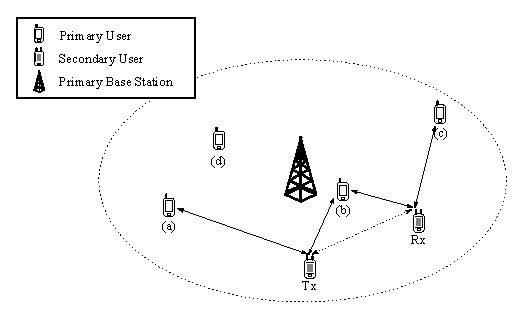
\includegraphics[scale=1]{Geo.eps}
\caption{Example of the system under study.}\label{fig:System}
\end{figure}

As an example, let us consider the system in Figure \ref{fig:System}, representing the coverage area (cell) of a PU base station (PU BS), where a cognitive pair (CP), consisting of an SU transmitter (SU Tx) and an SU receiver (SU Rx), tries to perform an SU transmission on a spectrum opportunity within this PU cell. Figure \ref{fig:System} also depicts the interference links between the SUs and the PU terminals. Because the SUs are within the range of the PU BS, there is also one interference link from the PU BS to each SU.
Before transmitting, both the SU Tx and the SU Rx scan the licensed spectrum looking for available channels and exchange control messages containing their sensing outcomes over a dedicated control channel.
Once the CP makes the access decision, the SU Tx starts the SU transmission over one or more available channels. It is assumed that the SU transmits in PU downlink channels. Although the BD scheme could be used for PU uplink channels, it is more effective for downlink channels for the reasons explained in Section \ref{BD_sec_results}.
The SU transmission is divided into time-slots. At the end of each time-slot, the SU Rx submits a control message to the SU Tx over the control channel. In general, this message would contain an ACK (or NACK) of the data transmitted on the time-slot, but our proposal will also include information about the power received at the SU Rx during the time-slot.

It is assumed that the signal power received at the SU Rx remains constant during a symbol time $T_{s}$ of the SU Tx transmission. In this case, the probability of correct signal detection at the SU Rx is defined in terms of the probability that the signal to interference ratio (SINR) is above a given threshold, which is determined by the minimum acceptable bit error rate (BER) for correct decoding, the transmission rate and the modulation used. Let us consider that, given the SU data packet length, and the information and redundancy bits in it, SU packets are correctly received if the BER during the packet reception is above certain value (e.g. $10^{-3}$). This BER objective is attained when the ratio $E_{b}/N_{0}$ is above a threshold $\gamma_{b}$, where $E_{b}$ is the energy per bit and $N_{0}$ is the noise spectral density (including both thermal and interference noise). The threshold depends on the modulation used (e.g. for BPSK, BER = $10^{-3}$ for $\gamma_{b}=7$ dB). Therefore, the threshold in terms of SINR is given by $\gamma = \gamma_{b}/(BT_{b})$ where $B$ is the channel bandwidth and $T_{b}$ the bit duration.

\subsection{Principles of the Background Detection Scheme}
Each SU data packet may be received at the SU Rx with or without PU interference. Let $P$ denote the signal power at the SU Rx during the reception of an SU data packet. The SU signal is received with power $Y$ at the SU Rx and, in case of transmission overlap, the signal transmitted by the PU BS is received with power $X$ at the SU Rx. Note that $P$, $X$, and $Y$ are random variables. Under PU-SU transmission overlap, $P=X+Y$ and, in absence of overlap, $P=Y$. Similarly, the SINR is $\text{\ttfamily{SINR}}=\frac{Y}{N+X}$, with overlap, and $\text{\ttfamily{SINR}}=\frac{Y}{N}$ without opverlap, where $N$ denotes the total thermal noise power in the channel bandwidth. If $\text{\ttfamily{SINR}}>\gamma$ the packet is correctly received and, if $\text{\ttfamily{SINR}}\leq\gamma$ the packet is impossible to decode (error event). 

After the reception of an SU data packet, the SU Rx can obtain two observations: $P$, and the occurrence (or absence) of an error event. The idea of the background detection (BD) mechanism is to use these observations to allow the SUs estimate the presence of PU activity during SU transmissions. If PU activity is detected, the OSA algorithm may decide to end the ongoing SU transmission to protect from interference any PU terminal in range of the SU Tx (In Figure \ref{fig:System}, PU terminals a and b) in case any of them is receiving PU BS transmissions on the channel where the overlap was detected.

The BD scheme is essentially a binary hypothesis testing mechanism conducted during SU transmission to decide on the most feasible value of a random variable $\Theta$, which takes two possible values $\left\{0,1\right\}$ at each SU packet reception. The event $\Theta = 1$ indicates that there has been PU interference during the packet reception, and $\Theta = 0$ indicates that the reception was free of PU interference.
%whether or not there has been PU interference during the reception of an SU data packet. These two hypotheses are referred to as $H_{1}$ (PU activity) and $H_{0}$ (no PU activity). 
The probability density functions (PDF) of $Y$ and $X$ are $f_{Y}(y)$ and $f_{X}(x)$ respectively. In case that both the SU Tx and the PU BS signals experience Rayleigh fading over their respective links to the SU Rx, we have 
\begin{align}{lcl}
f_{Y}(y) & = & \displaystyle\frac{1}{p_{ss}}e^{-\frac{y}{p_{ss}}}\\
f_{X}(x) & = & \displaystyle\frac{1}{p_{ps}}e^{-\frac{x}{p_{ps}}} 
\end{align}
where $p_{ss}$ is the average power received from the SU Tx and $p_{ps}$ is the average power received from the PU BS. Both distributions, as well as the average powers can be obtained from the previous sensing history of the SUs. 
Similarly, this sensing history provides information about the PU traffic profile and intensity on the scanned channels.
One basic metric is the probability of PU activity during the transmission time of an SU packet ($\mathbold{P}\left(\Theta = \theta\right)$), with $\theta = \left\{0,1\right\}$.
Therefore, assuming $f_{Y}(y)$, $f_{X}(x)$ and $\mathbold{P}\left(\Theta = \theta\right)$ are known, the hypothesis testing is based on Bayesian estimation, resulting in a maximum a posteriori probability (MAP) decision rule. In Section \ref{BD_sec_results} we evaluate the sensitivity of the BD mechanism to the inaccuracies in the estimation of the PDFs and traffic parameters.

Summarizing, once the SU transmission has started, the SU Rx obtains, upon each packet reception, the following observation:
\begin{equation}
\left(P,E\right) = 
\begin{cases}
\left(p_{r},0\right) &,\mbox{if }\text{\ttfamily{SINR}}>\gamma\\
\left(p_{r},1\right) &,\mbox{if }\text{\ttfamily{SINR}}\leq\gamma
\end{cases}
\end{equation}
And, upon this observation, the MAP decision rule selects the hypothesis having the maximum posterior distribution over the two possible values of $\theta$. Next section provides a detailed derivation for the BD MAP rule, and obtains the probabilities of correct and incorrect detection of the MAP estimator.

%The effect of inaccuracies on the distribution estimation will be addressed in Section \ref{BD_sec_results}. 

%Modelo de transmision
%PU tx sincronizado time-slots
%SU transmision. En el downlink del PU. 1 scanning time-slot. Several tx time slots. ACK en cada time-slot.
%Problema de interferencia.

%Modelo de errores. Fading lento. SINR por bit.

%Propueta Background Detection.
%Observacion P y E.
%A partir de ellas se puede realizar un test de hipotesis.


\section{PU Activity Detection in Background}\label{sec:Detection}
\subsection{MAP Rule}\label{sec:MAPrule}
Given the observation pair, $\left(P=p_{r},E=e\right)$, the MAP rule selects the hypothesis $H_{i}$ for which the posterior probability $\mathbold{P}\left(\Theta=\theta|P=p_{r},E=e\right)$ is largest. 
By Bayes' rule this is equivalent to select the hypothesis maximizing $p_{\Theta}\left(\theta\right)f_{P,E|\Theta}\left(p_{r},e|\theta\right)$.
Because $E$ is a discrete random variable, we have to consider separately each possible value of the outcome $e$ ($e=0$, if the SU packet is received without errors and $e=1$ otherwise) for the computation of the posterior probability. Let $E_{0}$ and $E_{1}$ refer to the events $e=0$ and $e=1$ respectively. Similarly, we use $H_{0}$ and $H_{1}$ to refer to the events $\Theta=0$ and $\Theta=1$.
Let us derive the expression of $f_{P,E|\Theta}\left(p_{r},e|\theta\right)$ for each possible combination of $E_{0}$ and $E_{1}$ with $H_{0}$ and $H_{1}$.

\subsubsection{Case $E_{1}$, $H_{1}$} Applying the definitions we have
\begin{equation}\label{definitionE1H1}
\begin{array}{lcl}
f_{P,E_{1}|H_{1}}\left(p_{r},E_{1}|H_{1}\right) & = & \displaystyle\frac{\partial}{\partial p_{r}}\mathbold{P}\left(P\leq p_{r},\text{\ttfamily{SINR}} \leq \gamma | H_{1}\right)\\
&= & \displaystyle\frac{\partial}{\partial p_{r}}\mathbold{P}\left(X+Y\leq p_{r},Y\leq N\gamma+X\gamma\right)
\end{array}
\end{equation}
We will first find the joint PDF of $P$ and $X$ and then integrate to find the PDF of $P$.
\begin{equation}\label{PxE1H1}
\begin{array}{lcl}
\mathbold{P}\left(X+Y\leq p_{r},Y\leq N\gamma+X\gamma|X=x\right) & = & \mathbold{P}\left(Y\leq p_{r}-x,Y\leq N\gamma+x\gamma|X=x\right)\\
& = &\mathbold{P}\left(Y\leq \text{min}\left(p_{r}-x,N\gamma+x\gamma\right)|X=x\right)\\
& = &\mathbold{P}\left(Y\leq \text{min}\left(p_{r}-x,N\gamma+x\gamma\right)\right)\\
& = & \displaystyle\int_{-\infty}^{\text{min}\left(p_{r}-x,N\gamma+x\gamma\right)}f_{Y}(y)dy\\
& = &
\begin{cases}
\displaystyle\int_{-\infty}^{p_{r}-x}f_{Y}(y)dy &,\mbox{if }p_{r}\leq N\gamma+x\left(\gamma+1\right)\\
\displaystyle\int_{-\infty}^{N\gamma+x\gamma}f_{Y}(y)dy &,\mbox{otherwise }
\end{cases}
\end{array}
\end{equation}
where the third equality comes from the independence of the PU and SU signals, $X$ and $Y$. By differentiating both sides with respect to $p_{r}$ we obtain
\begin{equation}\label{fxE1H1}
f_{P,E_{1}|H_{1},X}\left(p_{r},E_{1}|H_{1},x\right) =
\begin{cases}
f_{Y}\left(p_{r}-x\right) &,\mbox{if }p_{r}\leq N\gamma+x\left(\gamma+1\right)\\
0 &,\mbox{otherwise }
\end{cases}
\end{equation}
Then, the joint PDF of $P$ and $X$ is
\begin{equation}\label{jointE1H1}
\begin{array}{lcl}
f_{P,X,E_{1}|\Theta}\left(p_{r},x,E_{1}|H_{1}\right) & = & f_{X|\Theta}\left(x|H_{1}\right)f_{P,E_{1}|\Theta}\left(p_{r},E_{1}|H_{1}\right)\\
& = & f_{X}\left(x\right)f_{P,E_{1}|\Theta}\left(p_{r},E_{1}|H_{1}\right)\\
& = &
\begin{cases}
f_{X}\left(x\right)f_{Y}\left(p_{r}-x\right) &,\mbox{if }p_{r}\leq N\gamma+x\left(\gamma+1\right)\\
0 &,\mbox{otherwise }
\end{cases}
\end{array}
\end{equation}
from which we finally obtain
\begin{equation}\label{finalE1H1}
\begin{array}{lcl}
f_{P,E_{1}|H_{1}}\left(p_{r}\right) & = & \displaystyle\int_{-\infty}^{\infty}f_{P,X,E_{1}|\Theta}\left(p_{r},x,E_{1}|H_{1}\right)dx\\
& = &
\displaystyle\int_{\frac{p_{r}-N\gamma}{\left(1+\gamma\right)}}^{\infty}f_{X}\left(x\right)f_{Y}\left(p_{r}-x\right)dx %\displaystyle\int_{\text{max}\left(0,\frac{p_{r}-N\gamma}{\left(1+\gamma\right)}\right)}^{\infty}f_{X}\left(x\right)f_{Y}\left(p_{r}-x\right)dx
\end{array}
\end{equation}
where $f_{P,E_{1}|H_{1}}\left(p_{r}\right)$ denotes $f_{P,E_{1}|H_{1}}\left(p_{r},E_{1}|H_{1}\right)$ in a more compact form.
When both links are characterized by Rayleigh fading, $f_{X}\left(x\right)$ and $f_{Y}\left(y\right)$ are exponential distributions and we have
\begin{equation}\label{finalExponentialE1H1}
f_{P,E_{1}|H_{1}}\left(p_{r}\right) =
\begin{cases}
\displaystyle\frac{e^{-\frac{p_{r}}{p_{ps}}} - e^{\left(-\frac{p_{r}}{p_{ss}}+ \frac{\left(p_{ps}-p_{ss}\right)\left(p_{r}-N\gamma\right)}{p_{ps}p_{ss}\left(1+\gamma\right)} \right)} }{p_{ps}-p_{ss}} &,\mbox{if }p_{r}\geq N\gamma\\
\displaystyle\frac{e^{-\frac{p_{r}}{p_{ps}}} - e^{-\frac{p_{r}}{p_{ss}}}}{p_{ps}-p_{ss}} &,\mbox{otherwise }
\end{cases}
\end{equation}

\subsubsection{Case $E_{0}$, $H_{1}$} Proceeding similarly to the case above we have
\begin{equation}\label{definitionE0H1}
\begin{array}{lcl}
f_{P,E_{0}|H_{1}}\left(p_{r},E_{0}|H_{1}\right) & = & \displaystyle\frac{\partial}{\partial p_{r}}\mathbold{P}\left(P\leq p_{r},\text{\ttfamily{SINR}} > \gamma | H_{1}\right)\\
&= & \displaystyle\frac{\partial}{\partial p_{r}}\mathbold{P}\left(X+Y\leq p_{r},Y>N\gamma+X\gamma\right)
\end{array}
\end{equation}
To obtain the joint PDF of $X$ and $P$ we need the following probability
\begin{equation}\label{PxE0H1}
\begin{array}{lcl}
\mathbold{P}\left(X+Y\leq p_{r},Y>N\gamma+X\gamma|X=x\right) & = & \mathbold{P}\left(X+Y\leq p_{r},Y>N\gamma+X\gamma\right)\\
& = &\mathbold{P}\left(N\gamma+X\gamma < Y\leq p_{r}-x \right)\\
& = &
\begin{cases}
\displaystyle\int_{N\gamma+X\gamma}^{p_{r}-x}f_{Y}(y)dy &,\mbox{if }x<\frac{p_{r}-N\gamma}{1+\gamma}\\
0 &,\mbox{otherwise }
\end{cases}
\end{array}
\end{equation}
By differentiating with respect to $p_{r}$ we obtain
\begin{equation}\label{fxE0H1}
f_{P,E_{0}|H_{1},X}\left(p_{r},E_{0}|H_{1},x\right) =
\begin{cases}
\displaystyle\frac{\partial}{\partial p_{r}}\displaystyle\int_{N\gamma+X\gamma}^{p_{r}-x}f_{Y}(y)dy &,\mbox{if }x<\frac{p_{r}-N\gamma}{1+\gamma}\\
0 &,\mbox{otherwise }
\end{cases}
\end{equation}
Then, after obtaining the joint PDF of $X$ and $P$, we integrate over $x$ to get
\begin{equation}\label{finalE0H1}
f_{P,E_{0}|H_{1}}\left(p_{r}\right) = \displaystyle\int_{-\infty}^{\frac{p_{r}-N\gamma}{1+\gamma}}\left(\displaystyle\frac{\partial}{\partial p_{r}}\displaystyle\int_{N\gamma+X\gamma}^{p_{r}-x}f_{Y}(y)dy\right) f_{X}(x)dx
\end{equation}
which, for Rayleigh fading has the following form
\begin{equation}\label{finalExponentialE0H1}
f_{P,E_{0}|H_{1}}\left(p_{r}\right) =
\begin{cases}
\displaystyle\frac{1}{p_{ps}-p_{ss}}e^{-\frac{p_{r}}{p_{ss}}} \left(e^{\frac{\left(p_{ps}-p_{ss}\right)\left(p_{r}-N\gamma\right)}{p_{ps}p_{ss}\left(1+\gamma\right)}} -1 \right) &,\mbox{if }p_{r}> N\gamma\\
0 &,\mbox{otherwise }
\end{cases}
\end{equation}

\subsubsection{Case $E_{1}$, $H_{0}$} In this case there is no signal received from the PU and the conditional PDF of $P$ is defined as follows
\begin{equation}\label{definitionE1H0}
\begin{array}{lcl}
f_{P,E_{1}|H_{0}}\left(p_{r},E_{1}|H_{1}\right) & = & \displaystyle\frac{\partial}{\partial p_{r}}\mathbold{P}\left(P\leq p_{r},\text{\ttfamily{SINR}} \leq \gamma | H_{1}\right)\\
&= & \displaystyle\frac{\partial}{\partial p_{r}}\mathbold{P}\left(Y\leq p_{r},Y\leq N\gamma\right)
\end{array}
\end{equation}
The probability in the right hand side is given by
\begin{equation}\label{PxE1H0}
\begin{array}{lcl}
\mathbold{P}\left(Y\leq p_{r},Y\leq N\gamma\right) & = & \mathbold{P}\left(Y\leq\text{min}\left(p_{r},N\gamma\right)\right)\\
& = &
\begin{cases}
\displaystyle\int_{-\infty}^{p_{r}}f_{Y}(y)dy &,\mbox{if }p_{r}\leq N\gamma\\
\displaystyle\int_{-\infty}^{N\gamma}f_{Y}(y)dy &,\mbox{otherwise }
\end{cases}
\end{array}
\end{equation}
By differentiating with respect to $p_{r}$ we obtain
\begin{equation}\label{finalE1H0}
f_{P,E_{1}|H_{0}}\left(p_{r}\right) = 
\begin{cases}
f_{Y}(p_{r}) &,\mbox{if }p_{r}\leq N\gamma\\
0 &,\mbox{otherwise }
\end{cases}
\end{equation}
The expression for Rayleigh fading is straightforward.

\subsubsection{Case $E_{0}$, $H_{0}$} The PDF of $P$ is now given by
\begin{equation}\label{definitionE0H0}
\begin{array}{lcl}
f_{P,E_{0}|H_{0}}\left(p_{r},E_{0}|H_{1}\right) & = & \displaystyle\frac{\partial}{\partial p_{r}}\mathbold{P}\left(P\leq p_{r},\text{\ttfamily{SINR}}>\gamma | H_{1}\right)\\
&= & \displaystyle\frac{\partial}{\partial p_{r}}\mathbold{P}\left(Y\leq p_{r},Y>N\gamma\right)
\end{array}
\end{equation}
where $\mathbold{P}\left(Y\leq p_{r},Y>N\gamma\right)$ equals $\mathbold{P}\left(N\gamma<Y\leq p_{r}\right)$ when $p_{r}> N\gamma$ and is 0 otherwise. Therefore we have
%\begin{equation}\label{PxE0H0}
%\mathbold{P}\left(Y\leq p_{r},Y\leq N\gamma\right) =
%\begin{cases}
%\displaystyle\int_{N\gamma}^{p_{r}}f_{Y}(y)dy &,\mbox{if }p_{r}\geq N\gamma\\
%0 &,\mbox{otherwise }
%\end{cases}
%\end{equation}
%And $f_{P,E_{0}|H_{0}}\left(p_{r}\right)$ is 
\begin{equation}\label{finalE0H0}
f_{P,E_{0}|H_{0}}\left(p_{r}\right) = 
\begin{cases}
\displaystyle\frac{\partial}{\partial p_{r}}\displaystyle\int_{N\gamma}^{p_{r}}f_{Y}(y)dy &,\mbox{if }p_{r}> N\gamma\\
0 &,\mbox{otherwise }
\end{cases}
\end{equation}
The particularization for Rayleigh fading is straightforward.

Given the above expressions, the MAP rule is specified by partitioning the observation space into disjoint sets in which each of the two hypothesis is chosen. In case a reception error has occurred ($E_{1}$), the following equation provides the threshold value(s) for the received power
\begin{equation}\label{thresholdE1}
\mathbold{P}\left(H_{0}\right)f_{P,E_{1}|H_{0}}\left(p_{r}\right) = \mathbold{P}\left(H_{1}\right)f_{P,E_{1}|H_{1}}\left(p_{r}\right)
\end{equation}
And in the $E_{0}$ event, the corresponding equation is
\begin{equation}\label{thresholdE0}
\mathbold{P}\left(H_{0}\right)f_{P,E_{0}|H_{0}}\left(p_{r}\right) = \mathbold{P}\left(H_{1}\right)f_{P,E_{0}|H_{1}}\left(p_{r}\right)
\end{equation}

Let us determine the power thresholds for the case of Rayleigh fading. 
Considering exponential distributions for $X$ and $Y$ in (\ref{thresholdE1}), we obtain the following two equations for $E_{1}$
\begin{align}{lccl}
\mathbold{P}\left(H_{0}\right)\cdot0 & = & \mathbold{P}\left(H_{1}\right)\displaystyle\frac{e^{-\frac{p_{r}}{p_{ps}}} - e^{\left(-\frac{p_{r}}{p_{ss}}+ \frac{\left(p_{ps}-p_{ss}\right)\left(p_{r}-N\gamma\right)}{p_{ps}p_{ss}\left(1+\gamma\right)} \right)} }{p_{ps}-p_{ss}} &,\mbox{if }p_{r}>N\gamma \label{E1ThresholdEq1} \\
\mathbold{P}\left(H_{0}\right)\displaystyle\frac{e^{-\frac{p_{r}}{p_{ss}}}}{p_{ss}}& = & \mathbold{P}\left(H_{1}\right)\displaystyle\frac{e^{-\frac{p_{r}}{p_{ps}}} - e^{-\frac{p_{r}}{p_{ss}}}}{p_{ps}-p_{ss}} &,\mbox{if }p_{r}\leq N\gamma \label{E1ThresholdEq2}
\end{align}
The first equation (\ref{E1ThresholdEq1}) only holds for $p_{r}=\infty$. Therefore, whenever $p_{r}>N\gamma$, the MAP rule selects the hypothesis $H_{1}$, which is rational because if $p_{r}>N\gamma$, the hypothesis $H_{0}$ implies that $\text{\ttfamily{SINR}}>\gamma$ which is inconsistent with $E_{1}$. In other words, if $p_{r}>N\gamma$, $E_{1}$ is caused by PU interference. 
It can be checked that the solution of second equation (\ref{E1ThresholdEq2}) is
\begin{equation}
p^{*} = \displaystyle\frac{p_{ss}p_{ps}}{p_{ps}-p_{ss}}\text{log}\left(\displaystyle\frac{p_{ps}-p_{ss}}{p_{ss}}\displaystyle\frac{\mathbold{P}\left(H_{0}\right)}{\mathbold{P}\left(H_{1}\right)}+1\right)
\end{equation}
If $p^{*}$ is a real number and $p^{*}\leq N\gamma$, then $p^{*}_{E_{1}}$ = $p^{*}$ is the threshold below which the MAP rule selects the hypothesis $H_{0}$ in the event $E_{1}$. In case (\ref{E1ThresholdEq2}) has no solution in $\left(0,N\gamma\right]$, then $p^{*}_{E_{1}}$ = $N\gamma$ if the left hand side of (\ref{E1ThresholdEq2}) is larger than the right hand side, and $p^{*}_{E_{1}}$ = 0 otherwise.

Considering Rayleigh fading, the equation for $E_{0}$, (\ref{thresholdE0}) results in the following two equations
\begin{align}{lccl}
\mathbold{P}\left(H_{0}\right)\displaystyle\frac{e^{-\frac{p_{r}}{p_{ss}}}}{p_{ss}} & = & \mathbold{P}\left(H_{1}\right)\displaystyle\frac{e^{-\frac{p_{r}}{p_{ss}}} \left(e^{\frac{\left(p_{ps}-p_{ss}\right)\left(p_{r}-N\gamma\right)}{p_{ps}p_{ss}\left(1+\gamma\right)}}-1\right)}{p_{ps}-p_{ss}} &,\mbox{if }p_{r}>N\gamma \label{E0ThresholdEq1} \\
\mathbold{P}\left(H_{0}\right)\cdot0 & = & \mathbold{P}\left(H_{1}\right)\cdot0 &,\mbox{if }p_{r}\leq N\gamma \label{E0ThresholdEq2}
\end{align}
The second equation (\ref{E0ThresholdEq2}) is trivially held for every $p_{r}\leq N\gamma$ because it corresponds to an unfeasible event: the absence of error when $p_{r}\leq N\gamma$ i.e. when $\text{\ttfamily{SINR}}\leq\gamma$. For $p_{r}>N\gamma$ equation (\ref{E0ThresholdEq1}) has the following solution
\begin{equation}
p^{*} =  \displaystyle\frac{p_{ss}p_{ps}\left(1+\gamma\right)}{p_{ps}-p_{ss}}\left(\text{log}\left(\displaystyle\frac{p_{ps}-p_{ss}}{p_{ss}}\displaystyle\frac{\mathbold{P}\left(H_{0}\right)}{\mathbold{P}\left(H_{1}\right)}+1\right)+\displaystyle\frac{N\gamma\left(p_{ps}-p_{ss}\right)}{p_{ss}p_{ps}\left(1+\gamma\right)}\right)
\end{equation}
If $p^{*}$ is a real number and $p^{*}>N\gamma$, then $p^{*}_{E_{0}}$ = $p^{*}$ is the threshold above which the MAP rule selects the hypothesis $H_{1}$ in the event $E_{0}$. Otherwise one of the two hypothesis always holds. The threshold is defined as $p^{*}_{E_{0}}$ = $N\gamma$ if $H_{1}$ always holds or as $p^{*}_{E_{0}}$ = $\infty$ if $H_{0}$ always holds.

We have therefore determined four disjoint sets in the observation space:
%NOTA: INSERTAR UNA FIGURA AQU� PUEDE FACILITAR LA LECTURA DEL PAPER
\begin{align}{lcl}
R_{H_{0}E_{0}} & = & \left\{\left(p_{r},e\right):p_{r} \leq p^{*}_{E_{0}}, e=0\right\}\\ 
R_{H_{1}E_{0}} & = & \left\{\left(p_{r},e\right):p_{r} > p^{*}_{E_{0}}, e=0\right\}\\ 
R_{H_{0}E_{1}} & = & \left\{\left(p_{r},e\right):p_{r} \leq p^{*}_{E_{1}}, e=1\right\}\\ 
R_{H_{1}E_{1}} & = & \left\{\left(p_{r},e\right):p_{r} > p^{*}_{E_{1}}, e=1\right\}
\end{align}
When $X$ and $Y$ are not described by exponential distributions, the procedure to determine the $R_{H_{i}E_{j}}$ sets is analogous to the one described. These sets are not only useful to establish the MAP rule, but also to estimate the probabilities of correct or incorrect detection. 
\subsection{Detection Probability}\label{sec:ErrorEstimation}
For each possible combination of $H_{0}$, $H_{1}$ and $E_{0}$, $E_{1}$, two outcomes of the MAP estimation are possible, $\hat{H}_{0}$, $\hat{H}_{1}$, corresponding to the hypothesis $\hat{\theta}=0$ and $\hat{\theta}=1$ respectively. Selecting $\hat{H}_{1}$ when $H_{0}$ is true is generally referred to as a Type I error, and selecting $\hat{H}_{0}$ when $H_{1}$ is true is a Type II error.

Let us first consider the analysis of the probabilities for $H_{1}$, i.e. when transmission overlap is present. The probability of a Type II error when the SU packet is received correctly is defined as
\begin{equation}
\mathbold{P}(\hat{H}_{0},E_{0}|H_{1}) = \mathbold{P}\left(\left(P,E\right)\in R_{H_{0}E_{0}}|H_{1}\right),
\end{equation}
the probability of correct PU activity detection when the SU packet is received correctly is
\begin{equation}
\mathbold{P}(\hat{H}_{1},E_{0}|H_{1}) = \mathbold{P}\left(\left(P,E\right)\in R_{H_{1}E_{0}}|H_{1}\right),
\end{equation}
the Type II error probability when the SU packet received is erroneous is 
\begin{equation}
\mathbold{P}(\hat{H}_{0},E_{1}|H_{1}) = \mathbold{P}\left(\left(P,E\right)\in R_{H_{0}E_{1}}|H_{1}\right),
\end{equation}
and the probability of correct PU activity detection when the SU packet received is erroneous is
\begin{equation}
\mathbold{P}(\hat{H}_{1},E_{1}|H_{1}) = \mathbold{P}\left(\left(P,E\right)\in R_{H_{1}E_{1}}|H_{1}\right),
\end{equation}

Let us obtain these probabilities for sets $R_{H_{i}E_{j}}$ defined with two thresholds ($p^{*}_{E_{0}}$ and $p^{*}_{E_{1}}$) and then particularize for Rayleigh fading.
The probability $\mathbold{P}(\hat{H}_{0},E_{0}|H_{1})$ is given by
\begin{equation}\label{PH0E0H1}
\begin{array}{lcl}
\mathbold{P}(\hat{H}_{0},E_{0}|H_{1}) & = & \mathbold{P}\left(P\leq p^{*}_{E_{0}}, \text{\ttfamily{SINR}}>\gamma|H_{1}\right)\\
& = & \mathbold{P}\left(X+Y\leq p^{*}_{E_{0}},Y>N\gamma+X\gamma\right)\\
& = & \mathbold{P}\left(N\gamma+X\gamma<Y\leq p^{*}_{E_{0}}-X\right)\\
& = & \displaystyle\int_{0}^{x^{*}}\displaystyle\int_{N\gamma+x\gamma}^{p^{*}_{E_{0}}-x}f_{Y}(y)f_{X}(x)dydx
\end{array}
\end{equation}
where 
\begin{equation}
x^{*} = \displaystyle\frac{p^{*}_{E_{0}}-N\gamma}{\gamma+1}
\end{equation}
Solving for $X$ and $Y$ exponentially distributed we obtain the following probability
\begin{equation}
\mathbold{P}(\hat{H}_{0},E_{0}|H_{1}) = e^{-\frac{x^{*}}{p_{ps}}}p_{ss}
\displaystyle\frac{e^{\frac{p^{*}_{E_{0}}}{p_{ss}}} ( e^{-\frac{x^{*}}{p_{ss}}} - e^{\frac{x^{*}}{p_{ps}}} )}{p_{ss}-p_{ps}} +
\displaystyle\frac{e^{-\frac{\left(\left(N+x^{*}\right)\gamma\right)}{p_{ss}}} 
( e^{x^{*}\left(\frac{1}{p_{ps}}+\frac{\gamma}{p_{ss}}\right)} - 1 )}{p_{ss}-p_{ps}\gamma}
\end{equation}
The probability of correct PU detection at the $E_{0}$ event is obtained as follows
\begin{equation}\label{PH1E0H1}
\begin{array}{lcl}
\mathbold{P}(\hat{H}_{1},E_{0}|H_{1}) & = & \mathbold{P}\left(P>p^{*}_{E_{0}}, \text{\ttfamily{SINR}}>\gamma|H_{1}\right)\\
& = & \mathbold{P}\left(X+Y>p^{*}_{E_{0}},Y>N\gamma+X\gamma\right)\\
& = & \mathbold{P}\left(Y>\text{max}\left(p^{*}_{E_{0}}-X,N\gamma+X\gamma\right)\right)\\
& = & \displaystyle\int_{0}^{x^{*}}\displaystyle\int_{p^{*}_{E_{0}}-x\gamma}^{\infty}f_{Y}(y)f_{X}(x)dydx +
\displaystyle\int_{x^{*}}^{\infty}\displaystyle\int_{N\gamma+x\gamma}^{\infty}f_{Y}(y)f_{X}(x)dydx
\end{array}
\end{equation}
The expression for Rayleigh fading is
\begin{equation}
\mathbold{P}(\hat{H}_{1},E_{0}|H_{1}) = \frac{e^{-\frac{p^{*}_{E_{0}}}{p_{ss}}} \left(-1+e^{\left(\frac{1}{p_{ss}}-\frac{1}{p_{ps}}\right) x^{*}}\right) p_{ss}}{p_{ps}-p_{ss}}+\frac{e^{-\frac{x^{*}}{p_{ss}}-\frac{\gamma(N+x^{*})}{p_{ss}}} p_{ss}}{p_{ss}+p_{ps}\gamma}
\end{equation}
The probability Type II error at the $E_{1}$ event is given by
\begin{equation}\label{PH0E1H1}
\begin{array}{lcl}
\mathbold{P}(\hat{H}_{0},E_{1}|H_{1}) & = & \mathbold{P}\left(P\leq p^{*}_{E_{1}}, \text{\ttfamily{SINR}}\leq\gamma|H_{1}\right)\\
& = & \mathbold{P}\left(X+Y\leq p^{*}_{E_{1}},Y\leq N\gamma+X\gamma\right)\\
& = & \mathbold{P}\left(Y\leq\text{min}\left(N\gamma+X\gamma,p^{*}_{E_{1}}-X\right)\right)\\
& = & \mathbold{P}\left(Y\leq p^{*}_{E_{1}}-X\right)\\
& = & \displaystyle\int_{0}^{p^{*}_{E_{1}}}\displaystyle\int_{0}^{p^{*}_{E_{1}}-x}f_{Y}(y)f_{X}(x)dydx
\end{array}
\end{equation}
where the last equality comes from the fact that $p^{*}_{E_{1}}\leq N\gamma$. The expression for Rayleigh fading is
\begin{equation}
\mathbold{P}(\hat{H}_{0},E_{1}|H_{1}) = \frac{p_{ps}\left(1-e^{-\frac{p^{*}_{E_{1}}}{p_{ps}}}\right)+\left(-1+e^{-\frac{p^{*}_{E_{1}}}{p_{ss}}}\right) p_{ss}}{p_{ps}-p_{ss}}
\end{equation}

The probability correct PU activity detection at $E_{1}$ is
\begin{equation}\label{PH1E1H1}
\begin{array}{lcl}
\mathbold{P}(\hat{H}_{1},E_{1}|H_{1}) & = & \mathbold{P}\left(P>p^{*}_{E_{1}}, \text{\ttfamily{SINR}}\leq\gamma|H_{1}\right)\\
& = & \mathbold{P}\left(X+Y>p^{*}_{E_{1}},Y\leq N\gamma+X\gamma\right)\\
& = & \mathbold{P}\left(p^{*}_{E_{1}}-X<Y\leq N\gamma+X\gamma\right)\\
& = & \displaystyle\int_{0}^{p^{*}_{E_{1}}}\displaystyle\int_{p^{*}_{E_{1}}-x }^{N\gamma+x\gamma}f_{Y}(y)f_{X}(x)dydx + 
\displaystyle\int_{p^{*}_{E_{1}}}^{\infty}\displaystyle\int_{0}^{N\gamma+x\gamma}f_{Y}(y)f_{X}(x)dydx
\end{array}
\end{equation}
For Rayleigh fading the expression of this probability is
\begin{equation}
\mathbold{P}(\hat{H}_{1},E_{1}|H_{1})= \frac{e^{-\frac{p^{*}_{E_{1}}}{p_{ps}}} p_{ps}}{p_{ps}-p_{ss}}+\frac{e^{-\frac{p^{*}_{E_{1}}}{p_{ss}}} p_{ss}}{-p_{ps}+p_{ss}}-\frac{e^{-\frac{N \gamma}{p_{ss}}} p_{ss}}{p_{ss}+p_{ps}\gamma}
\end{equation}
It can be checked that $\sum_{i:0,1}\sum_{j:0,1}\mathbold{P}(\hat{H}_{i},E_{j}|H_{1})=1$.
Figure \ref{fig:Regions} illustrates the integration regions for the detection probabilities under transmission overlap.

\begin{figure}[ht]
\centering
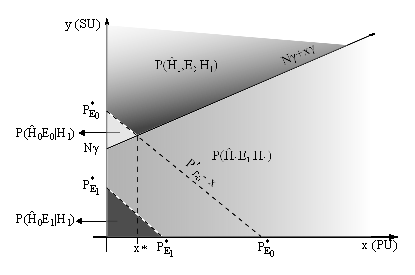
\includegraphics[scale=1]{Regions.eps}
\caption{Integration regions to compute probabilities of correct detection, type I and type II errors under the $H_{1}$ event (transmission overlap).}\label{fig:Regions}
\end{figure}

Let us now obtain the probabilities for $H_{0}$, i.e. in absence of transmission overlap. The probabilities are defined in the following way
\begin{align}{lcl}
\mathbold{P}(\hat{H}_{0},E_{0}|H_{0}) & = & \mathbold{P}\left(\left(P,E\right)\in R_{H_{0}E_{0}}|H_{0}\right)\\
\mathbold{P}(\hat{H}_{1},E_{0}|H_{0}) & = & \mathbold{P}\left(\left(P,E\right)\in R_{H_{1}E_{0}}|H_{0}\right)\\
\mathbold{P}(\hat{H}_{0},E_{1}|H_{0}) & = & \mathbold{P}\left(\left(P,E\right)\in R_{H_{0}E_{1}}|H_{0}\right)\\
\mathbold{P}(\hat{H}_{1},E_{1}|H_{0}) & = & \mathbold{P}\left(\left(P,E\right)\in R_{H_{0}E_{1}}|H_{0}\right)
\end{align}
We now obtain these probabilities as in the $H_{1}$ case. 
The correct estimation probability $\mathbold{P}(\hat{H}_{0},E_{0}|H_{0})$ is given by
\begin{equation}\label{PH0E0H0}
\begin{array}{lcl}
\mathbold{P}(\hat{H}_{0},E_{0}|H_{0}) & = & \mathbold{P}\left(P\leq p^{*}_{E_{0}},\text{\ttfamily{SINR}}>\gamma|H_{0}\right)\\
& = & \mathbold{P}\left(Y\leq p^{*}_{E_{0}},Y>N\gamma\right)\\
& = & \mathbold{P}\left(N\gamma<Y\leq p^{*}_{E_{0}}\right)\\
& = & \displaystyle\int_{N\gamma}^{p^{*}_{E_{0}}}f_{Y}(y)dy
\end{array}
\end{equation}
which, in the case of Rayleigh fading equals $e^{-N\gamma/p_{ss}}-e^{-p^{*}_{E_{0}}/p_{ss}}$.
The Type I error $\mathbold{P}(\hat{H}_{0},E_{0}|H_{0})$ is 
\begin{equation}\label{PH1E0H0}
\begin{array}{lcl}
\mathbold{P}(\hat{H}_{1},E_{0}|H_{0}) & = & \mathbold{P}\left(P>p^{*}_{E_{0}}, \text{\ttfamily{SINR}}>\gamma|H_{0}\right)\\
& = & \mathbold{P}\left(Y>p^{*}_{E_{0}},Y>N\gamma\right)\\
& = & \mathbold{P}\left(Y>\text{max}\left(p^{*}_{E_{0}},N\gamma\right)\right)\\
& = & \mathbold{P}\left(Y>p^{*}_{E_{0}}\right)\\
& = & \displaystyle\int_{p^{*}_{E_{0}}}^{\infty}f_{Y}(y)dy
\end{array}
\end{equation}
For Rayleigh fading $\mathbold{P}(\hat{H}_{1},E_{0}|H_{0})=e^{-p^{*}_{E_{0}}/p_{ss}}$.
The correct estimation probability at the $E_{1}$ event is
\begin{equation}\label{PH0E1H0}
\begin{array}{lcl}
\mathbold{P}(\hat{H}_{0},E_{1}|H_{0}) & = & \mathbold{P}\left(P\leq p^{*}_{E_{1}}, \text{\ttfamily{SINR}}\leq\gamma|H_{0}\right)\\
& = & \mathbold{P}\left(Y\leq p^{*}_{E_{1}},Y\leq N\gamma\right)\\
& = & \mathbold{P}\left(Y\leq\text{min}\left(N\gamma+X\gamma,p^{*}_{E_{1}}\right)\right)\\
& = & \mathbold{P}\left(Y\leq p^{*}_{E_{1}}\right)\\
& = & \displaystyle\int_{0}^{p^{*}_{E_{1}}}f_{Y}(y)dy
\end{array}
\end{equation}
which for Rayleigh fading is $1-e^{-p^{*}_{E_{1}}/p_{ss}}$. Finally the Type I error probability at the $E_{1}$ event is
\begin{equation}\label{PH1E1H0}
\begin{array}{lcl}
\mathbold{P}(\hat{H}_{1},E_{1}|H_{0}) & = & \mathbold{P}\left(P>p^{*}_{E_{1}}, \text{\ttfamily{SINR}}\leq\gamma|H_{0}\right)\\
& = & \mathbold{P}\left(Y>p^{*}_{E_{1}},Y\leq N\gamma\right)\\
& = & \mathbold{P}\left(p^{*}_{E_{1}}<Y\leq N\gamma\right)\\
& = & \displaystyle\int_{p^{*}_{E_{1}}}^{N\gamma}f_{Y}(y)dy
\end{array}
\end{equation}
which equals $e^{-p^{*}_{E_{1}}/p_{ss}}-e^{-N\gamma/p_{ss}}$ for Rayleigh fading.

\section{Markov Model for Optimized OSA}\label{sec:Markov}
In this section, we analyze the use of the proposed background detection (BD) mechanism in an OSA system maximizing the SU throughput subject to constraints on the collision probability with PU transmissions.
We assume single-channel transmission capabilities for the SU, leaving for future research the generalization to the multiple-channel case.
An SU transmission period consists of one scanning slot followed by $N$ consecutive time-slots. The SU detects at least one available channel during the scanning slot, otherwise this scanning slot does not corresponds to a scanning slot. After the scanning slot, the SU transmits one data packet in each one of the $N$ remaining time-slots of the SU transmission period.
Note that $N$ denotes, in general, a random variable. However, as later explained, this is only the case for OSA with BD.
Two parameters characterize the system performance: the SU throughput ($T$), defined as the expected number of correctly received SU packets per time-slot in an SU transmission period, and the collision probability $P_{c}$, defined as the PU-SU transmission overlap probability per time-slot in a SU transmission period.

PU inter arrival time follows a geometric distribution as well as the channel holding time, i.e. the equivalent of a Poisson traffic model for discrete-time. In every time-slot, a channel free of PU traffic is occupied by a PU transmission with probability $p$, and an ongoing PU transmission ends with probability $q$.
The SU uses estimations of $p$ and $q$ to optimize the duration of the transmission period under collision probability constraints.
The effect that the estimation inaccuracies in both the traffic intensity and in the traffic model have in the OSA performance is addressed in Section \ref{BD_sec_results}.

Considering the $n$-th time-slot of an SU transmission period, $\phi_{n}$ denotes the probability vector for PU activity in the channel during this time-slot. In the single-channel traffic model considered, $\phi_{n}$ contains two elements: $\phi_{n}(1)$ and $\phi_{n}(2)$, corresponding to no PU activity and PU activity in the channel respectively. The probability vector in the scanning slot is $\phi_{0} = (1,0)$ if the detection is perfect. With imperfect sensing, $\phi_{0} = (1-p_{\bar{n}},p_{\bar{n}})$, where $p_{\bar{n}}$ denotes the probability of false negative (the sensing outcome indicates that the channel is free of PU activity when it is not). Given the transition matrix of the Markov model for the PU activity in the channel, $M=\left[\begin{smallmatrix}1-p&p\\q&1-q\end{smallmatrix}\right]$, the probability vector for the $n$-th time-slot is given by $\phi_{n}' = M^{n}\phi_{n}'$, where ``$'$'' stands for the transpose operation.

\subsection{OSA Without Background Detection}
In this case, after the scanning slot, the SU transmits in the channel during a fixed number of slots.
In an optimized OSA, this number maximizes $T$ while $P_{c}$ remains below a given value $\alpha$. Let $T(n)$ and $P_{c}(n)$ denote $T$ and $P_{c}$ as functions of $n$. The optimized OSA selects a number of time-slots solving the following problem
\begin{equation}
\underset{n}{\mbox{max }} T(n)\mbox{ subject to }P_{c}(n) \leq \alpha
\end{equation}
which is solved for nonnegative integers $n$ up to a maximum value $n_{\text{m}}$, which stands for avoiding unbounded $n$ in case $T(n)$ attains its maximum at $n\rightarrow\infty$ and $P_{c}(n)$ remains under $\alpha$ for every $n$. Note that, provided that $\phi_{0} = (1,0)$, $P_{c}(n)$ is a monotonically increasing sequence bounded by $p/(p+q)$. If several values of $n$ attain the maximum, the OSA algorithm picks the one with the lowest $P_{c}$. We refer to this value as $n^{*}$.

The expression for $P_{c}(n)$ is given by
\begin{equation}
P_{c}(n) = \displaystyle\frac{1}{n+1}\displaystyle\sum_{i=1}^{n}\phi_{i}(2)
\end{equation}

Defining $\mathbold{P}(E_{0}|H_{0})$ as the probability of correctly receiving an SU packet in the absence of collision, and $\mathbold{P}(E_{0}|H_{1})$ as the probability of $E_{0}$ in a time-slot with collision, $T(n)$ is given by the following equation
\begin{equation}
T(n) = \displaystyle\frac{1}{n+1}\left[\displaystyle\sum_{i=1}^{n}\phi_{i}(1)\mathbold{P}(E_{0}|H_{0}) + \displaystyle\sum_{i=1}^{n}\phi_{i}(2)\mathbold{P}(E_{0}|H_{1})\right]
\end{equation}
The probability $\mathbold{P}(E_{0}|H_{0})$ is obtained as follows
\begin{equation}\label{PE0H0}
\begin{array}{lcl}
\mathbold{P}(E_{0}|H_{0}) & = & \mathbold{P}\left(\text{\ttfamily{SINR}}>\gamma|H_{0}\right)\\
& = & \mathbold{P}\left(Y>N\gamma\right)\\
& = & \displaystyle\int_{N\gamma}^{\infty}f_{Y}(y)dy
\end{array}
\end{equation}
%The reception error probability under collision is 
and $\mathbold{P}(E_{0}|H_{1})$ is given by
\begin{equation}\label{PE0H1}
\begin{array}{lcl}
\mathbold{P}(E_{0}|H_{1}) & = & \mathbold{P}\left(\text{\ttfamily{SINR}}>\gamma|H_{1}\right)\\
& = & \mathbold{P}\left(Y>N\gamma+X\gamma\right)\\
& = & \displaystyle\int_{0}^{\infty}\displaystyle\int_{N\gamma+x\gamma}^{\infty}f_{Y}(y)f_{X}(x)dydx
\end{array}
\end{equation}
For Rayleigh fading we have 
\begin{align}{lcl}
\mathbold{P}(E_{0}|H_{0}) & = & e^{-\frac{N\gamma}{p_{ss}}}\\
\mathbold{P}(E_{0}|H_{1}) & = & \displaystyle\frac{p_{ss}e^{-\frac{N\gamma}{p_{ss}}}}{p_{ss} + p_{ps}\gamma}
\end{align}

\subsection{OSA With Background Detection}
In contrast to previous scheme, when OSA includes BD, the duration of the SU transmission period is not deterministic. Because BD can detect PU activity simultaneously to SU packet reception, the SU transmission can be aborted at any time-slot.
Figure \ref{fig:Slots} compares a transmission period without BD with two possible outcomes of the transmission period using BD. Case (a) is the standard SU transmission period when the BD scheme does not detect PU activity in any slot. Case (b) corresponds to the case when the BD scheme detects a PU transmission is a slot, resulting in the immediate termination of the SU transmission in this channel.

\begin{figure}[ht]
\centering
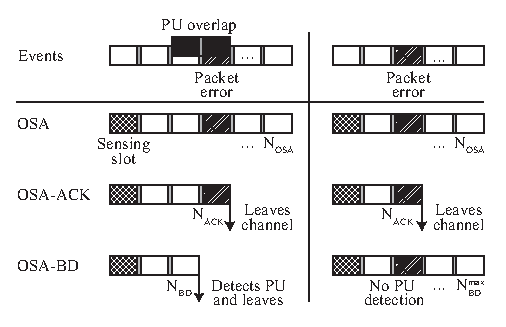
\includegraphics[scale=1]{Slots.eps}
\caption{Transmission periods with and without BD. When using BD the transmission period can be aborted if PU activity is detected during an SU transmission slot. Inter-slot periods are required for signaling.}\label{fig:Slots}
\end{figure}

In order to compute $T$ and $P_{c}$ we develop a Markov-reward model of the SU transmission process, consisting in a discrete-time Markov chain (DTMC) in which each state is associated to a reward defined in terms of $T$ of $P_{c}$, depending on what is being computed.
The DTMC, denoted by $Z_{k}$, characterizes a process of consecutive SU transmissions, where $k$ enumerates time-slots. 
The integer value $i$ taken by $Z_{k}$. i.e. the state of the DTMC at the $k$-th time-slot, has the following interpretation:
\begin{itemize}
	\item If $i$ is odd, the channel is free of PU activity (${H}_{0}$) at the $\left\lceil i/2\right\rceil$-th time-slot.
	\item If $i$ is even, the channel presents PU activity (${H}_{1}$) at the $i/2$-th time-slot.
\end{itemize}
After the scanning time-slot ($i=0$), the SU transmits with probability $1$, and enters state $i=1$ with probability $1-p$ and state $i=2$ with probability $p$.
The DTMC advances to a higher state if the BD does not detect PU activity ($\hat{H}_{0}$), and returns to state 0 otherwise, which means the end of the ongoing SU transmission.
Therefore, the DTMC transition probabilities are defined as
\begin{equation}
\begin{array}{lcll}\label{BD_eq_transition_prob}
p_{0,1} & = & 1-p &\\
p_{0,2} & = & p &\\
p_{2k-1,2k+1} & = & (1-p)\mathbold{P}(\hat{H}_{0}|H_{0}) &,\mbox{ for } 0<k<n\\
p_{2k-1,2k+2} & = & p\mathbold{P}(\hat{H}_{0}|H_{0}) &,\mbox{ for } 0<k<n\\
p_{2k-1,0} & = & 1-\mathbold{P}(\hat{H}_{0}|H_{0}) &,\mbox{ for } 0<k<n\\
p_{2k,2k+1} & = & q\mathbold{P}(\hat{H}_{0}|H_{1}) &,\mbox{ for } 0<k<n\\
p_{2k,2k+2} & = & (1-q)\mathbold{P}(\hat{H}_{0}|H_{1}) &,\mbox{ for } 0<k<n\\
p_{2k,0} & = & 1-\mathbold{P}(\hat{H}_{0}|H_{1}) &,\mbox{ for } 0<k<n\\
p_{n,0} & = & 1 &
\end{array}
\end{equation}
where $\mathbold{P}(\hat{H}_{0}|H_{0})$ and $\mathbold{P}(\hat{H}_{0}|H_{1})$ can be obtained as follows
\begin{equation}
\begin{array}{lcl}
\mathbold{P}(\hat{H}_{0}|H_{0}) & = & \mathbold{P}(\hat{H}_{0},E_{0}|H_{0}) + \mathbold{P}(\hat{H}_{0},E_{1}|H_{0})\\
\mathbold{P}(\hat{H}_{0}|H_{1}) & = & \mathbold{P}(\hat{H}_{0},E_{0}|H_{1}) + \mathbold{P}(\hat{H}_{0},E_{1}|H_{1})
\end{array}
\end{equation}
where $\mathbold{P}(\hat{H}_{0},E_{0}|H_{1})$, $\mathbold{P}(\hat{H}_{0},E_{1}|H_{1})$, $\mathbold{P}(\hat{H}_{0},E_{0}|H_{0})$, and $\mathbold{P}(\hat{H}_{0},E_{1}|H_{0})$, are obtained by (\ref{PH0E0H1}), (\ref{PH0E1H1}), (\ref{PH0E0H0}), and (\ref{PH0E1H0})respectively.
Figure \ref{fig:Markov} depicts the graph of the DTMC.

\begin{figure}[ht]
\centering
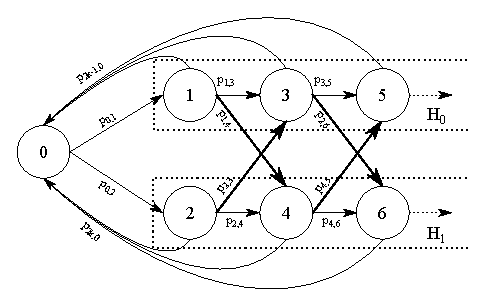
\includegraphics[scale=1]{Markov.eps}
\caption{Graph of the DTMC characterizing the SU transmission process.}\label{fig:Markov}
\end{figure}

%thus entering state $i=1$. At any state $i>0$ the chain may return to state $i=0$ if the BD detects PU activity, or may advance to state $i+1$ if the BD does not detect PU activity. In order to establish a bound on $P_{c}$ it is necessary to define a limit $n$ on the number of consecutive SU transmissions. As in previous subsection, $n$ is set to the optimal value $n^{*}=\text{arg max}_{n}T(n)$ s.t. $P_{c}(n) \leq \alpha$.

For a generic reward $r(i)$, the expected average reward is defined as 
$\bar{r} = \underset{K\rightarrow\infty}{\text{lim }}\frac{1}{K}\sum_{k = 0}^{K}r\left(Z_{k}\right)$. For an ergodic, finite-state Markov chain, and provided that $\left|r\left(i\right)\right|$ is bounded for every $i$, the total expected average reward $\bar{r}$ is $\bar{r} = \sum_{i = 0}^{n}r\left(i\right)\pi_{i}$, where $\pi_{i}$ are the steady state probabilities of the DTMC obtained by solving the equilibrium equations $\boldsymbol{\pi} = \boldsymbol{\pi}\mathbold{T}$, $\left\|\boldsymbol{\pi}\right\| = \displaystyle\sum_{i=0}^{n}\pi_{i}=1$, where $\mathbold{T}$ is the transition matrix containing the probabilities defined in (\ref{BD_eq_transition_prob}). Let $r_{T}(i)$ and $r_{P_{c}}(i)$ denote the per-state reward for computing $T$ and $P_{c}$ respectively. According to the definitions of $T$ and $P_{c}$, and because the DTMC models consecutive SU transmissions, $\bar{r}_{T} = T$ and $\bar{r}_{P_{c}} = P_{c}$. We will use the terms $\bar{r}_{T}(n)$ and $\bar{r}_{P_{c}}(n)$ to refer to the SU throughput and collision probability when using BD and the maximum length of SU transmissions is set to $n$ time-slots. The optimal $n$ is obtained by solving the following optimization problem
\begin{equation}
\underset{n}{\mbox{max }} \bar{r}_{T}(n)\mbox{ subject to }\bar{r}_{P_{c}}(n) \leq \alpha
\end{equation}
which is solved for integers $n \in \left\{0,1,\ldots,n_{\text{m}}\right\}$. 
Note that the trivial values for $n=0$ are $\bar{r}_{T}(0)=0$ and $\bar{r}_{P_{c}}(0)=0$. 
If there are more than one solution, the optimal transmission limit $n^{*}$ is the lowest one attaining the maximum throughput.

Let us see how to obtain $r_{T}(i)$ and $r_{P_{c}}(i)$ for every $i$. The per-stage throughput $r_{T}(i)$ is defined as the expected number of SU packets correctly received at the $i$-th SU transmission time-slot. By definition, for every $i>0$, the SU transmits one packet, therefore $r_{T}(i) = \mathbold{P}(E_{0}|i)\cdot1$, where $\mathbold{P}(E_{0}|i)$ is the probability of the $E_{0}$ event at the $i$-th time-slot, and is given by
\begin{equation}
\mathbold{P}(E_{0}|i) =
\begin{cases}
\mathbold{P}(E_{0}|H_{0}) &,\mbox{if }i\mbox{ odd}\\
\mathbold{P}(E_{0}|H_{1}) &,\mbox{if }i\mbox{ even}
\end{cases}
\end{equation}
%By applying the law of total probability we have
%\begin{equation}
%\begin{array}{lcl}
%r_{T}(i) & = & \mathbold{P}(E_{0}|i)\\
%& = & \mathbold{P}(E_{0}|H_{0})\mathbold{P}(H_{0}|i) + \mathbold{P}(E_{0}|H_{1})\mathbold{P}(H_{1}|i)\\
%& = & \mathbold{P}(E_{0}|H_{0})\phi_{i}(1) + \mathbold{P}(E_{0}|H_{1})\phi_{i}(2)
%\end{array}
%\end{equation}
for $i>0$, where $\mathbold{P}(E_{0}|H_{0})$ and $\mathbold{P}(E_{0}|H_{1})$ are given by (\ref{PE0H0}) and (\ref{PE0H1}) respectively. Similarly, the per-stage collision probability is $r_{P_{c}}(i)~=~0$ when $i$ is odd, and $r_{P_{c}}(i)~=~1$ when $i$ is even. For $i=0$ we have $r_{T}(0)~=~0$ and $r_{P_{c}}(0)~=~0$. 

The specific structure of matrix $\mathbold{T}$ allows an efficient computation of the steady-state probability vector $\boldsymbol{\pi}$. Let us express $\mathbold{T}$ in a block-matrix form
\begin{equation}
\mathbold{T} =
\begin{pmatrix}
			\textbf{B}_{0,0} & \textbf{B}_{0,1}  & \textbf{0} & \textbf{0} & \cdots \textbf{0} \\
			\textbf{B} & \textbf{0} & \textbf{A} & \textbf{0} & \cdots \textbf{0} \\
			\textbf{B} & \textbf{0} & \textbf{0} & \textbf{A} & \cdots \textbf{0} \\
			\vdots & \vdots & \vdots & \vdots &  \vdots\\
			\textbf{1} & \textbf{0} & \textbf{0} & \textbf{0} & \cdots \textbf{A} \\
			\end{pmatrix}
\end{equation}
where $\textbf{B}_{0,0} = (0, 0)$, $\textbf{B}_{0,1} = ((1-p), p)$, and
\begin{equation}
\begin{array}{lcl}
\mathbold{A} & = &
\begin{pmatrix}
			(1-p)\mathbold{P}(\hat{H}_{0}|H_{0}) & p\mathbold{P}(\hat{H}_{0}|H_{0})\\
			q\mathbold{P}(\hat{H}_{0}|H_{1}) & (1-q)\mathbold{P}(\hat{H}_{0}|H_{1})\\
			\end{pmatrix}\\
\mathbold{B} & = &
\begin{pmatrix}
			1-\mathbold{P}(\hat{H}_{0}|H_{0})\\
			1-\mathbold{P}(\hat{H}_{0}|H_{1})\\
			\end{pmatrix}\\
\mathbold{1} & = &
\begin{pmatrix}
			1\\
			1\\
			\end{pmatrix}\\			
\end{array}
\end{equation}
Let us define $\boldsymbol{\pi}_{k}~=~(\pi_{2k-1}, \pi_{2k})$, denoting the probability of the events $H_{0}$ and $H_{1}$ at the $k$-th transmission slot. Applying the equilibrium equations we have $\pi_{0}~=~\sum_{k=1}^{n-1}\boldsymbol{\pi}_{j}\textbf{B} + \boldsymbol{\pi}_{n}\mathbold{1}$, $\boldsymbol{\pi}_{1}~=~\pi_{0}\textbf{B}_{0,1}$, and $\boldsymbol{\pi}_{k}$ can be expressed in the matrix-geometric form $\boldsymbol{\pi}_{k}~=~\boldsymbol{\pi}_{1}\mathbold{A}^{k-1}~=~\pi_{0}\textbf{B}_{0,1}\mathbold{A}^{k-1}$. The normalization condition is $\pi_{0}+\sum_{k=1}^{n-1}\boldsymbol{\pi}_{j}\textbf{1} + \boldsymbol{\pi}_{n}\mathbold{1}~=~1$, which combined with the equilibrium equations results in the following expression for $\pi_{0}$
\begin{equation}\label{pi_0_basic}
\pi_{0} = \displaystyle\frac{1}{2+\sum_{k=1}^{n-1}\textbf{B}_{0,1}\mathbold{A}^{k-1}(\mathbold{1}-\textbf{B})}
\end{equation}
Because $\mathbold{A}$ is strictly positive we know, by the Perron-Frobenius theorem, that it has one positive eigenvalue, with multiplicity 1, which is strictly higher than all other eigenvalues. Since the dimension of $\mathbold{A}$ is $2\times2$, it has only two eigenvalues and thus we conclude that $\mathbold{A}$ has two distinct eigenvalues, $\lambda_{1}$ and $\lambda_{2}$ (with their corresponding eigenvectors $\mathbold{e}_{1}$ and $\mathbold{e}_{2}$). This implies that $\mathbold{A}$ can be expressed as $\mathbold{A}~=~\mathbold{M}\boldsymbol\Lambda\mathbold{M}^{-1}$ where $\mathbold{M}~=~\left[\mathbold{e}_{1} \mathbold{e}_{2}\right]$ and $\boldsymbol\Lambda$ is a diagonal matrix containing $(\lambda_{1}, \lambda_{2})$ in its diagonal. Then
\begin{equation}
\mathbold{A}^{k-1} = 
\mathbold{M}\begin{pmatrix}
\lambda_{1}^{k-1}&0\\
0&\lambda_{2}^{k-1}
\end{pmatrix}
\mathbold{M}^{-1}
\end{equation}
which allows us to express (\ref{pi_0_basic}) in the following closed form
\begin{equation}
\pi_{0} = \left(2+\textbf{B}_{0,1}\mathbold{M}
\begin{pmatrix}
\frac{1-\lambda_{1}^{n-1}}{1-\lambda_{1}}&0\\
0&\frac{1-\lambda_{2}^{n-1}}{1-\lambda_{2}}
\end{pmatrix}
\mathbold{M}^{-1}(\mathbold{1}-\textbf{B})\right)^{-1}
\end{equation}
which enables an efficient computation of $\boldsymbol{\pi}_{k}~=~\pi_{0}\textbf{B}_{0,1}\mathbold{A}^{k-1}$, for $k = 1,\ldots,n$.
%and the matrix-geometric form of $\boldsymbol{\pi}_{k}$ as
%\begin{equation}
%\boldsymbol{\pi}_{k}=\pi_{0}\textbf{B}_{0,1}\mathbold{M}\begin{pmatrix}
%\lambda_{1}^{(k-1)}&0\\
%0&\lambda_{2}^{(k-1)}
%\end{pmatrix}
%\mathbold{M}^{-1}
%\end{equation}
%$\boldsymbol\Lambda~=~\left[\begin{pmatrix}\lambda_{1}&0\\0&\lambda_{2}\end{pmatrix}\right]$

\section{Numerical Results}\label{BD_sec_results}
\subsection{Parameter Setting}
To assess the impact of using BD on the performance and, especially, on the robustness of the OSA scheme, we consider a cognitive pair located within PU BS cell. The distance between the of PU BS and the SU Rx is $d_{ps}=1000$ m. The PU BS transmission power on each channel, $p_{p}$, is 20 dBm. The transmission antenna height is $h_{t} = 10$ m and the receiver is at $h_{r} = 1.5$ m. The transmission and reception antenna gains are $g_{t} = 4$ dB and $g_{r} = 2$ dB respectively. With these parameters, the average interference power at the SU receiver due to PU BS transmission is given by the pathloss equation
\begin{equation}
p_{ps} = \displaystyle\frac{p_{p}(h_{t}h_{r})^2g_{t}g_{r}}{d_{ps}^{-4}}
\end{equation}
which equals -70.5 dBm. Assuming that the SU Tx antenna height and gain are 1.5 m and 4 dB respectively and that the distance between SU Tx and the SU Rx is $d_{ss} =250$ m, we obtain $p_{ss} = -72.9$ dBm. Considering a channel bandwidth $B = 2$ MHz, and an SU Rx noise figure equal to 18 dB, the total noise power is $N = -103$ dBm. The cognitive pair transmits at a rate of 2 Mbit/s using BPSK modulation and, as explained in Section \ref{BD_sec_system}, each packet is assumed to arrive correctly if BER$<10^{-3}$, therefore the SINR threshold is $\gamma=7$ dB. The PU traffic parameters are $p = 10^{-3}$ and $q = 2\cdot10^{-3}$, resulting in an occupation probability $\mathbold{P}\left(H_{1}\right) = \frac{1}{3}$. With these parameters we obtain the following thresholds for Rayleigh fading: $p^{*}_{E_{0}} = -61.8$ dBm and $p^{*}_{E_{1}} = -95.9$ dBm. The type I and type II error probabilities are $\mathbold{P}(\hat{H}_{1}|H_{0}) = 2.65\cdot10^{-6}$ and $\mathbold{P}(\hat{H}_{0}|H_{1}) = 0.1026$ respectively. The main parameters are summarized in Table \ref{BD_table_parameters}.

\begin{table}
\begin{tabular}{|c|l|} \hline
\textbf{Parameter} & \textbf{Assigned value}\\\hline\hline
$p_{ss}$&-72.9 dBm\\\hline
$p_{ps}$&-70.5 dBm\\\hline
$N$&-103 dBm\\\hline
$\gamma$& 7 dBm\\\hline
$p$ & $10^{-3}$\\\hline
$q$ & $2\cdot10^{-3}$\\\hline
$\mathbold{P}\left(H_{1}\right)$ & 1/3\\\hline
$p^{*}_{E_{0}}$ & -61.8 dBm\\\hline
$p^{*}_{E_{1}}$ & -95.9 dBm\\\hline
$\mathbold{P}(\hat{H}_{1}|H_{0})$ & $2.65\cdot10^{-6}$\\\hline
$\mathbold{P}(\hat{H}_{0}|H_{1})$ & 0.1026\\\hline
\end{tabular}
\centering
\caption{Parameter setting of the reference scenario used in numerical evaluations}
\label{BD_table_parameters}
\end{table}
%Before evaluating the performance and robustness of optimized OSA with and without BD, 
Before evaluating the performance and robustness of optimally configured OSA with and without BD, it is interesting to assess how the performance parameters (throughput $T$ and collision probability $P_{c}$) vary with the optimization parameter $n$ (in time-slots). Figure \ref{fig:performance_n} shows the throughput and collision performance versus $n$ for both implementations. The values of $T$ and $P_{c}$ are obtained numerically and by simulation also, to validate the model. We can appreciate one of the main advantages of using BD: while $P_{c}$ increases almost linearly with $n$ when BD is not used, it does not surpass a notably low level when BD is used. The reason is that PU activity can be detected during SU transmission, implying the end of the transmission. Therefore, although $n$ determines the maximum duration of a SU transmission when BD is used, the expected duration is determined by the PU activity detection. When BD is not used, larger values of $n$ imply higher $P_{c}$ and lower $T$, because transmission overlap also degrades SU performance. Seeing this figure, one can anticipate that the BD implementation may be more robust against parameter estimation inaccuracies, than the one without BD.

\begin{figure}[ht]
\centering
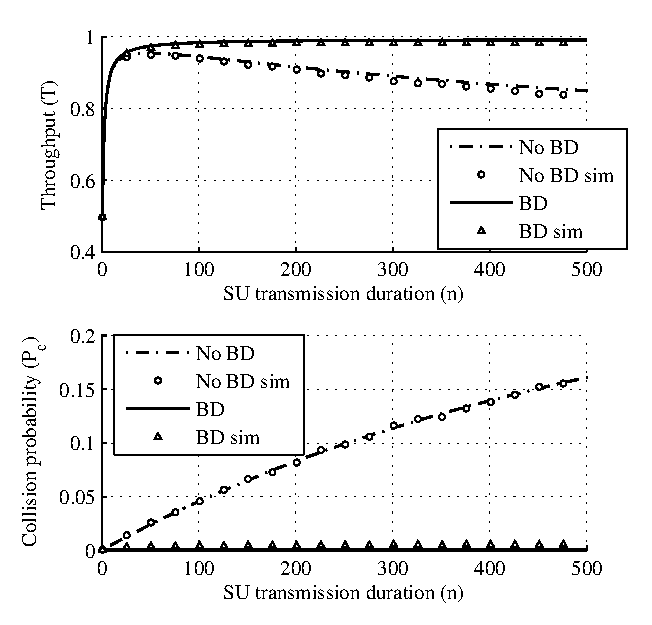
\includegraphics[scale=1]{PerformanceVSn_simulated.eps}
\caption[]{Throughput and collision performance with and without BS vs. the number of time-slots ($n$) of the SU transmission}\label{fig:performance_n}
\end{figure}
\subsection{Sensitivity to Estimation Inaccuracies}
In this subsection we study how the optimized implementations of OSA and OSA with BD perform under drifts of the real values of some critical parameters. 
By doing this, we evaluate the robustness of each implementation against inaccuracies on the parameter estimation. With the parameters described in previous subsection, and setting the collision probability threshold $\alpha = 0.025$, the optimal $n$ value for OSA without BD is 49. With BD, $T(n)$ increases monotonically with $n$, while $P(n)$ remains below 0.025. In this case we select $n=100$ which provides a throughput very close to the maximum, and would result in, at most, 0.05 collision probability in case of a complete malfunction of th BD mechanism.

Both schemes are heavily reliant on the characterization of the PU traffic in the channel. To evaluate the impact of traffic estimation inaccuracies, let us consider that the arrival traffic intensity $p$ differs from the estimated one $p_{\text{est}}$, which is used for the computation of $n^{*}$ in both schemes and for the threshold computation in BD. Figure \ref{fig:performance_estimationp} shows the performance versus the ratio $p/p_{\text{est}}$. We see that in both cases, the $T$ decreases and $P_{c}$ increases but, for the BD case the degradation is notably less severe than the no BD case, showing the higher robustness of BD against error in traffic estimation.

\begin{figure}[ht]
\centering
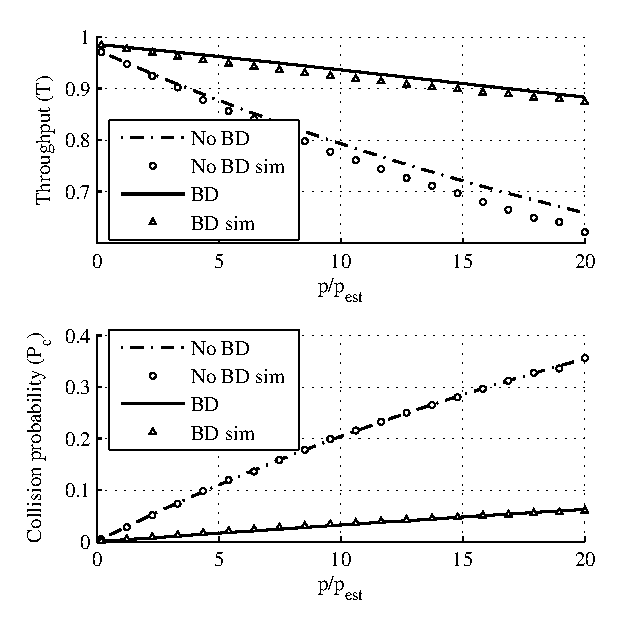
\includegraphics[scale=1]{PerformanceVsTrafficError_simulated.eps}
\caption[]{Throughput and collision performance with and without BS vs. the inaccuracy on the estimation of the traffic intensity}\label{fig:performance_estimationp}
\end{figure}

Another critical aspect in the BD scheme is the channel characterization. In the example developed, The MAP estimator is designed for a Rayleigh fading model for both PU and SU signals, assuming a previous knowledge of the average signal powers at the receiver. However it is possible that the SU misestimates the average power, especially for the PU signal ($p_{ps}$), or even the channel statistical description itself. To assess the effect of these misestimations, we have simulated an OSA system with BD configured for Rayleigh fading, to obtain the performance under different $p_{ps}$ estimation errors when the fading is Rayleigh, Ricean with $K=10$, and Nakagami with $m=2$. We also compare these results with the performance of an OSA system without BD in the same scenarios. As can be seen in Figure \ref{fig:performance_power}, OSA with BD maintains its advantage respect to the non BD system in almost every case. The statistical characterization of the fading shows a moderate impact on BD performance. In contrast, overestimating $p_{ps}$ shows to have the most harmful effect on the collision probability. The reason is that as the real $p_{ps}$ decreases respect the estimated value, the probability of Type II error approaches 1 and, in consequence the OSA with BD tends to operate as an OSA without BD. In Figure \ref{fig:performance_power}, OSA BD is set to $n = 100$ which, as explained previously, results in a $P_{c}$ near 0.05 in case of BD malfunctioning. If OSA and OSA BD are both configured with the same $n$ value, they present similar performance under $p_{ps}$ overestimation in the scenarios of Figure \ref{fig:performance_power}.
\begin{figure}[ht]
\centering
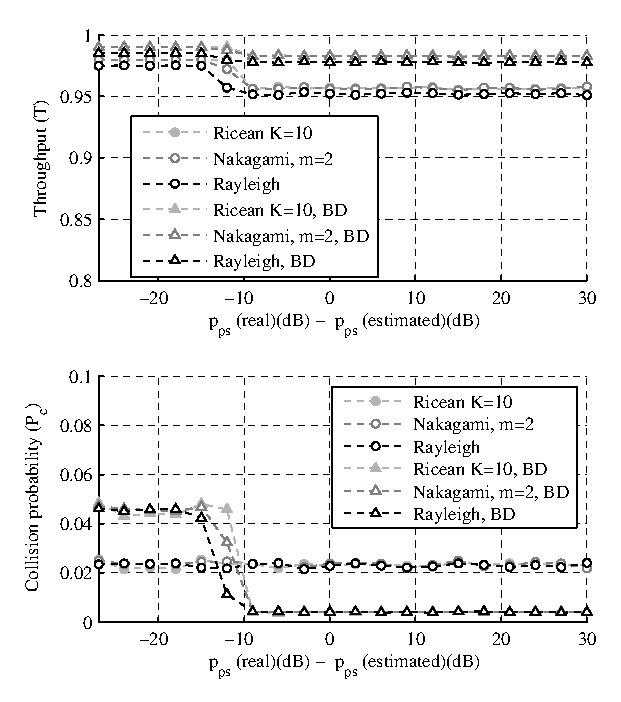
\includegraphics[scale=1]{PerformanceVsPower_simulated.eps}
\caption[]{Throughput and collision performance with and without BS vs. the inaccuracy on the estimation of the traffic intensity}\label{fig:performance_power}
\end{figure}
\section{Conclusions}\label{BD_sec_conclusion}
